% !TEX encoding = UTF-8
% !TEX TS-program = pdflatex
% !TEX root = ../tesi.tex

%**************************************************************
\chapter{I Microservizi}
%**************************************************************

%\epigraph{Citazione}{Autore della citazione}

\section{Architettura software}

Da quanto si può estrapolare dallo standard IEEE 1471-2000, il concetto di architettura software può essere definito come segue:
\begin{quotation}
	\noindent \textit{L'architettura software è l'organizzazione fondamentale delle componenti di un sistema, dalle relazioni che intercorrono tra esse e con l'ambiente, e i principi che ne governano la progettazione e l'evoluzione.}
\end{quotation} 

Esistono vari tipi di architettura software, ma il fine di questa sezione è quello di discutere le differenze, i pro e i contro tra un'architettura tradizionale monolitica e la ben più recente architettura a microservizi.

\clearpage

\subsection{Architettura monolitica}
Un prodotto software che adotta un'architettura monolitica, qualunque siano le sue dimensioni, può essere genericamente visto come l'immagine in figura  \ref{fig:monolithic-arch}:

\begin{figure}[H]
	\centering
	%	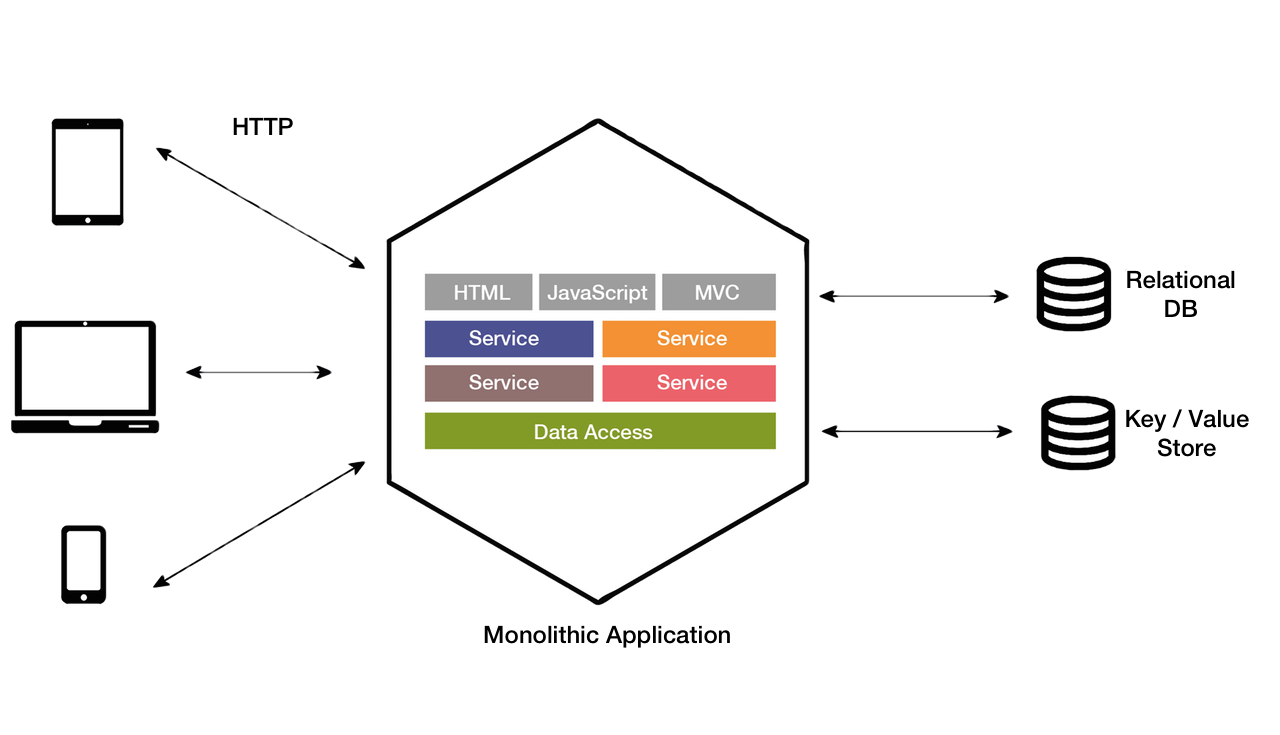
\includegraphics[width=\textwidth/2]{immagini/monolithic_architecture.png} % FONTE: https://medium.com
	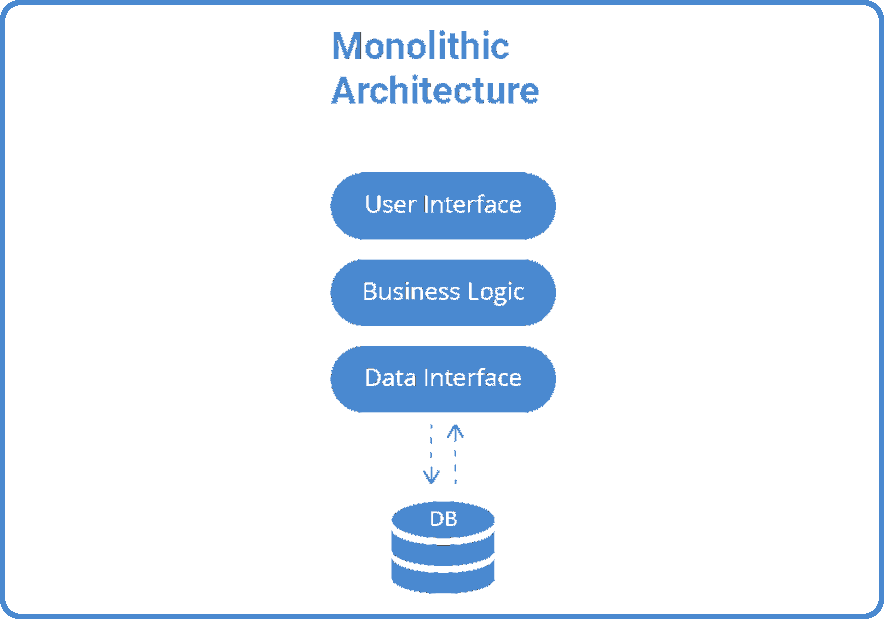
\includegraphics[width=0.28\textwidth]{immagini/monolithic_architectureB.png} % FONTE: https://www.sam-solutions.com/blog/microservices-vs-monolithic-real-business-examples/
	\caption[Architettura monolitica]{Architettura monolitica\footnotemark}
	\label{fig:monolithic-arch}
\end{figure}
\footnotetext{Fonte immagine: \href{https://www.sam-solutions.com/blog/microservices-vs-monolithic-real-business-examples/}{https://www.sam-solutions.com}}

Come è possibile notare dall'immagine, la \textit{business logic}, la gestione dei dati persistenti e la \textit{user interface}, sono racchiusi in un unico grande monolite, termine da cui è stato tratto il nome di questa architettura.

Che tipo di vantaggi può comportare adottare tale architettura?

% https://microservices.io/patterns/monolithic.html

\paragraph*{Sviluppo} Sviluppare un'applicazione monolitica è per natura semplice, poiché tutto ciò che serve è racchiuso in un unico, talvolta grande, progetto, e gli strumenti di sviluppo e/o IDE 
hanno un ottimo supporto in tale contesto.

\paragraph*{Deploy} Fare un \textit{deploy} dell'applicativo, ossia un rilascio, è banale e diretto, poiché è sufficiente ricompilare il progetto (se previsto dallo \textit{stack} tecnologico utilizzato) e rilasciarlo nell'ambiente di produzione.

\paragraph*{Facile da scalare} Per far scalare l'applicazione, è sufficiente farne girare copie multiple, con la possibilità di utilizzare un \textit{load balancer}.

\paragraph*{Testabilità} Facile da testare, poiché si ha il controllo di tutti gli input e gli output, con possibilità di \textit{mocking} dei \textit{layer}
non in fase di \textit{testing}

\bigskip
Veniamo ora agli svantaggi all'approccio monolitico.

\paragraph*{Dimensione intimidatoria} Al crescere delle dimensioni del progetto, diventa sempre più complicato individuare nuovi sviluppatori pronti ad apportare cambiamenti per nuove \textit{release},
viste le considerevoli dimensioni della \textit{code base}.
%Questo per via delle considerevoli dimensioni della \textit{code base}. che in applicazioni a livello \textit{enterprise} sono sempre di spessore non trascurabile.

\paragraph*{Continuous deployment} La pratica del \textit{continuous deployment} non è generalmente praticabile.
Per aggiornare un singolo componente, è necessario rilasciare l'intera applicazione, comportando minuti, se non ore, di totale indisponibilità del
servizio, nel suo complesso.
Per questo va effettuata una rigorosa pianificazione dei rilasci, nei periodi in cui l'applicativo viene usufruito di meno.

\paragraph*{Scalabilità} Mentre risulta facile scalare l'applicazione, non è altrettanto efficacie. Tutti i dati risiedono in un unico, potenzialmente
enorme, \textit{persistence layer}. Quando la mole di dati inizia ad essere
consistente, ogni componente, per ottenere i dati, deve passare attraverso quest'unico layer che comporta un alto traffico di IO, oltre che un attesa dovuta all'attesa del recupero dei dati dall'eventuale \textit{database}.

\paragraph*{Stack tecnologico} L'inizio dello sviluppo di un applicativo monolitico richiede un ``contratto'' a lungo termine con una stack tecnologico limitato. Una volta effettuata la scelta, non sarà possibile cambiare tecnologie per tutto il ciclo di vita del software (a meno che il prodotto non venga riscritto da zero), poiché tutte le componenti sono unite e dipendenti dalle tecnologie iniziali.

Gli svantaggi penalizzano molto fattori che riguardano la scalabilità
e progetti con target su grandi numeri.
Ecco perché negli ultimi anni il paradigma dei microservizi guadagna
sempre più popolarità ed è sulla bocca di tutti.

%\clearpage

% ------------------------------------------------------------------

\subsection{Architettura a microservizi}

Un'architettura a microservizi può essere genericamente vista come
nella figura che segue:

\begin{figure}[H]
	\centering
	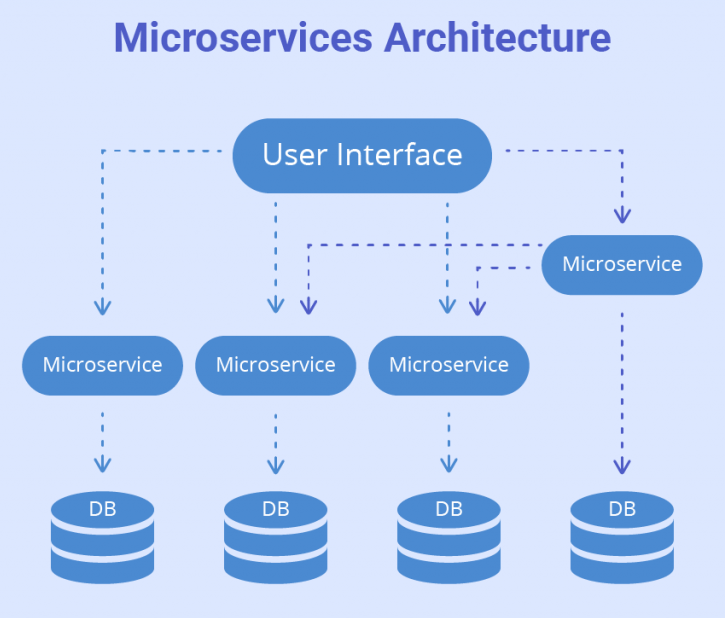
\includegraphics[width=0.8\textwidth]{immagini/microservices_architecture.png} % FONTE: https://www.sam-solutions.com/blog/microservices-vs-monolithic-real-business-examples/
	\caption[Architettura a microservizi]{Architettura  a microservizi\footnotemark}
	\label{fig:microservices-arch}
\end{figure}
\footnotetext{Fonte immagine: \href{https://www.sam-solutions.com/blog/microservices-vs-monolithic-real-business-examples/}{https://www.sam-solutions.com}}

In un'architettura a microservizi, 